\documentclass{article}

\usepackage{xeCJK}
\usepackage{tikz}
\usetikzlibrary{petri}
\usepackage{smartdiagram}
\usetikzlibrary{mindmap,trees}
\usetikzlibrary{calendar}
\usetikzlibrary{folding}
\usetikzlibrary{arrows.meta} % 自定义箭头样式
\usetikzlibrary{shapes.misc} % 图形库
\usetikzlibrary{shapes.geometric} % 图形库
\usetikzlibrary{shadings} % 渐变色
\usetikzlibrary{shadows} % 阴影
\usetikzlibrary{positioning} % 提供node的位置描述特性
\usetikzlibrary{lindenmayersystems}
\usepackage{xcolor}


\begin{document}
\section{图形}

\tikzstyle{sysBase} = [
  shape=rectangle, rounded corners=3mm,
  shade, ball color=green, drop shadow,
  text badly centered, inner sep=4mm]
\tikzstyle{sys1} = [
  sysBase, top color=blue, bottom color=blue, middle color=white
]
\tikzstyle{sys2} = [
  sysBase, top color=white, bottom color=blue,
]

\tikz{
  \node[sys1] (st1)  at (0,0) {\Huge{存储管理分系统}};
  \node[sys2, right=of st1] {\Huge{任务管理分系统}};   
  \node[sys1, below=of st1,left color=green, right color=green, middle color=white!80]  {应用处理子系统};  

}

\section{xcolor}
\definecolor{myc1}{rgb}{0.2,0.4,0.8}
\colorlet{myc12}{blue!10} % let myc12= rgb:0.5,0.1,0
\definecolorset{rgb}{x-}{-y}{red,1,0,0;green,0,1,0;blue,0,0,1}

\begin{testcolors}[rgb,cmyk,hsb,HTML,gray]
\testcolor{myc1}
\testcolor{myc12}
\testcolor{x-red-y}
\testcolor{x-green-y}
\testcolor{x-blue-y}
\testcolor{red!10!green!10!blue}
\testcolor{red!20!green!20!blue}
\testcolor{red!30!green!30!blue}
\testcolor{red!40!green!40!blue}
\testcolor{red!50!green!50!blue}
\testcolor{red!60!green!60!blue}
\testcolor{red!70!green!70!blue}
\testcolor{red!80!green!80!blue}
\testcolor{red!90!green!90!blue}
\testcolor{red}
\testcolor{red!75}
\testcolor{red!75!green}
\testcolor{red!75!green!50}
\testcolor{red!75!green!50!blue}
\testcolor{red!75!green!50!blue!25}
\testcolor{red!75!green!50!blue!25!gray}

\testcolor{rgb:red,4; green,4; blue,1}
\testcolor[hsb]{0.4,0.8,0.4}
\testcolor[cmyk]{0,0,.5,.5}
%\testcolor[rgb:cmyk]{0,0,.5,.5}
\end{testcolors}

\section{node}
\tikz{
  \node[draw,
    shape=isosceles triangle, % shape: circle, triangle
    fill=red,text=yellow
  ] at (0,0) {\Huge{ node style test}};

  \node[shade, top color=yellow,  bottom color=green, middle color=red % middle color must after top and bottom color
    ,shape=rectangle, rounded corners=1mm
    , scale=2] at (0,-4) {shade 1};

  \node[shade, left color=yellow, right color=green, middle color=red
    ,shape=rectangle, rounded corners=2mm
    , scale=2] at (4, -4) {shade 2};

  \node[shade, ball color=green
    ,shape=rectangle, rounded corners=3mm
    , scale=2] at (8, -4) {shade 3};

  \node[
    %% shade, ball color=green,
    shape=rectangle, rounded corners=3mm,
    draw, drop shadow={opacity=0.3},
    scale=2] at (0, -6) {shadow 1};

  \node[
    %shade, ball color=green,
    shape=rectangle, rounded corners=3mm,
    copy shadow, fill=green!20, draw=blue,
    scale=2] at (4, -6) {shadow 2};

  \node[draw=black,
    shape=circle, rounded corners=5mm,
    circular drop shadow,
    scale=2] at (8, -6) {shadow 3};
}
\tikz{
    % node tree;
  \node {node name}
  child {node {child node}}
  child {node {child node2}}
  ;
}


\section{Arrows}
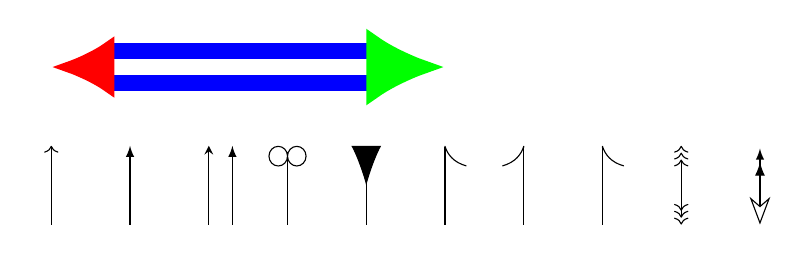
\begin{tikzpicture} [xxx /.tip={Latex[sep] latex[sep]},
    yyy /.tip={Stealth[length=10pt, open]}
  ]
  \draw [->] (0,0) -- (0, 1);
  \draw [-{stealth}] (2,0) -- (2,1);
  \draw [-{latex}] (1,0) -- (1,1);
  \draw [-latex] (2.3,0) -- (2.3, 1);
  \draw [arrows={-Hooks[arc=360, scale=3]}] (3,0) -- (3, 1); % 向左右然后向后弯曲的箭头,终点弯曲的角度为360度,360度就弯成圆圈了
  \draw [arrows={-Latex[reversed, scale=3]}] (4,0) -- (4,1); % 反向箭头
  \draw [arrows={->[harpoon, swap, scale=3]}] (5,0) -- (5,1); % harpoon箭头, swap研箭头方向为轴镜像
  \draw [arrows={->[left, scale=3]}] (6,0) -- (6,1); % 左半边
  \draw [arrows={->[right, scale=3]}] (7,0) -- (7,1); % 右半边
  \draw [<.<<->.>>] (8,0) -- (8,1);
  \draw [{yyy}-{xxx}] (9,0) -- (9,1);
  \draw [line width=2mm, double distance=2mm, color=blue,
    arrows={{Latex[width=8mm,length=8mm, color=red]}-{Latex[width=5mm,length=5mm, scale=2, color=green]}}
  ] (0,2) -- (5,2);
% [«.<-.»>] 
  
\end{tikzpicture}

\section{连线测试}
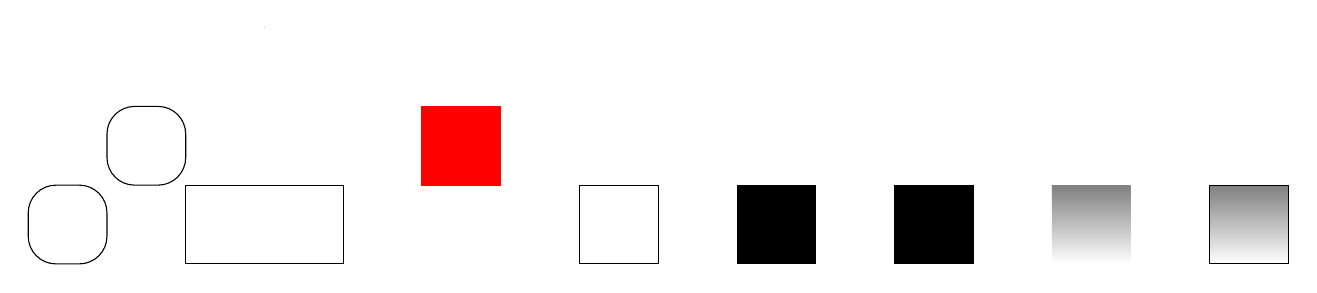
\begin{tikzpicture}
  \path [draw, rounded corners=10pt] (0,0) rectangle (1,1) (1,1) rectangle (2,2); % 多个path可以放在一行中写

  \path (4,1) rectangle (2,0) [draw]; % [] 参数的位置可以在开头,中间和结尾,建议结尾
  \path [draw] (5,1) rectangle (6,2) [fill, red] ; %参数可以分开写

  \draw (7,0) rectangle (8,1) ; % draw 表示画框线, fill表示填充
  \fill (9,0) rectangle (10,1);
  \filldraw (11,0) rectangle (12,1);
  \shade (13,0) rectangle (14,1); % shade 渐变?
  \shadedraw (15,0) rectangle (16,1);
  \clip (2,2) rectangle (3,3); % ?
  \useasboundingbox (4,2) rectangle (5,3);
  
  \draw [color=red, very thin] (3,3) rectangle (4,4);
  \node {root}
  child {node {no1}}
  child {node {no2}
    child {node {nxx1}}
    child {node {nxx2}}
  };
  
      
\end{tikzpicture}



\newpage
\section{神经网络图petriNet}
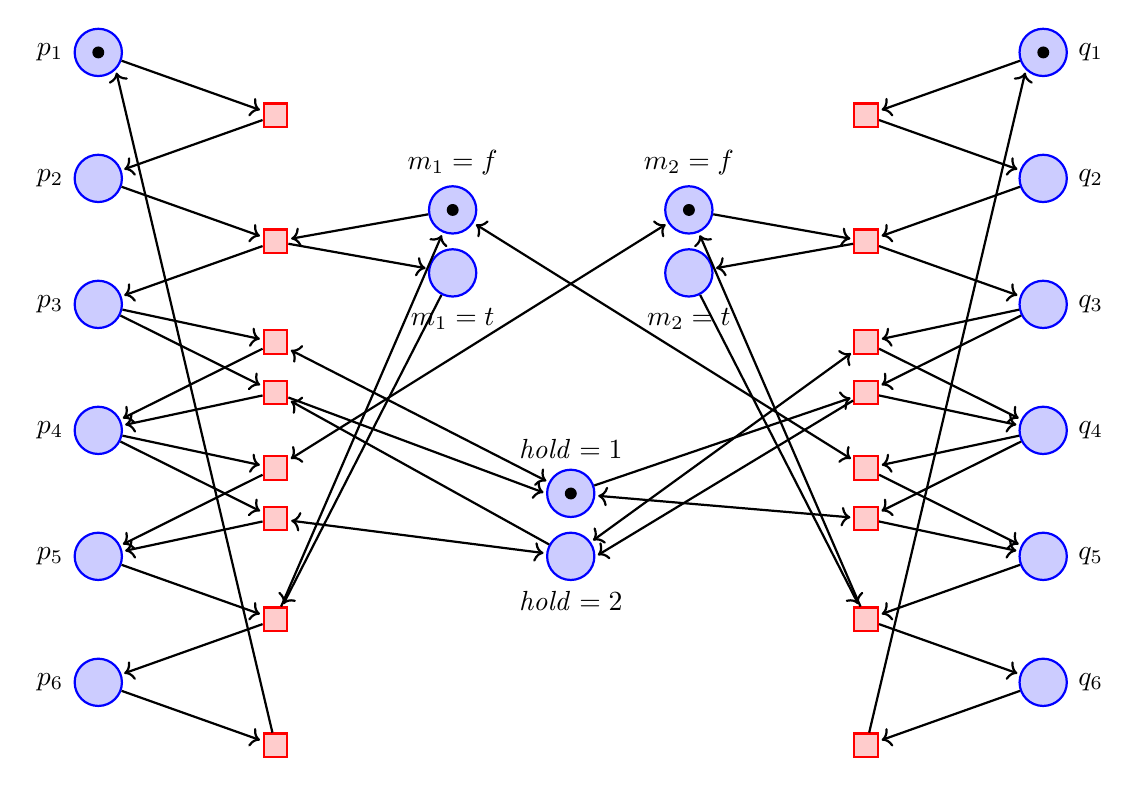
\begin{tikzpicture}[yscale=-1.6,xscale=1.5,thick,
every transition/.style={draw=red,fill=red!20,minimum size=3mm},
every place/.style={draw=blue,fill=blue!20,minimum size=6mm}]
\foreach \i in {1,...,6} {
\node[place,label=left:$p_\i$] (p\i) at (0,\i) {};
\node[place,label=right:$q_\i$] (q\i) at (8,\i) {};
}
\foreach \name/\var/\vala/\valb/\height/\x in
{m1/m_1/f/t/2.25/3,m2/m_2/f/t/2.25/5,h/\mathit{hold}/1/2/4.5/4} {
\node[place,label=above:{$\var = \vala$}] (\name\vala) at (\x,\height) {};
\node[place,yshift=-8mm,label=below:{$\var = \valb$}] (\name\valb) at (\x,\height) {};
}
\node[token] at (p1) {};
 \node[token] at (q1) {};
\node[token] at (m1f) {}; \node[token] at (m2f) {};
\node[token] at (h1) {};
\node[transition] at (1.5,1.5) {}
 edge
 [pre] (p1) edge [post] (p2);
\node[transition] at (1.5,2.5) {}
 edge
 [pre] (p2) edge[pre]
 (m1f)
edge
 [post](p3) edge[post] (m1t);
\node[transition] at (1.5,3.3) {}
 edge
 [pre] (p3) edge [post] (p4)
edge
 [pre and post] (h1);
\node[transition] at (1.5,3.7) {}
 edge
 [pre] (p3) edge [pre] (h2)
edge
 [post] (p4) edge [post] (h1.west);
\node[transition] at (1.5,4.3) {}
 edge
 [pre] (p4) edge [post] (p5)
edge
 [pre and post] (m2f);
\node[transition] at (1.5,4.7) {}
 edge
 [pre] (p4) edge [post] (p5)
edge
 [pre and post] (h2);
\node[transition] at (1.5,5.5) {}
 edge
 [pre] (p5) edge [pre] (m1t)
edge
 [post] (p6) edge [post] (m1f);
\node[transition] at (1.5,6.5) {}
 edge
 [pre] (p6) edge [post] (p1.south east);
\node[transition] at (6.5,1.5) {}
 edge
 [pre] (q1) edge [post] (q2);
\node[transition] at (6.5,2.5) {}
 edge
 [pre] (q2) edge [pre] (m2f)
edge
 [post] (q3) edge [post] (m2t);
\node[transition] at (6.5,3.3) {}
 edge
 [pre] (q3) edge [post] (q4)
edge
 [pre and post] (h2);
\node[transition] at (6.5,3.7) {}
 edge
 [pre] (q3) edge [pre] (h1)
edge
 [post] (q4) edge [post] (h2.east);
\node[transition] at (6.5,4.3) {}
 edge
 [pre] (q4) edge [post] (q5)
edge
 [pre and post] (m1f);
\node[transition] at (6.5,4.7) {}
 edge
 [pre] (q4) edge [post] (q5)
edge
 [pre and post] (h1);
\node[transition] at (6.5,5.5) {}
 edge
 [pre] (q5) edge [pre] (m2t)
edge
 [post] (q6) edge [post] (m2f);
\node[transition] at (6.5,6.5) {}
 edge
 [pre] (q6) edge [post] (q1.south west);
\end{tikzpicture}

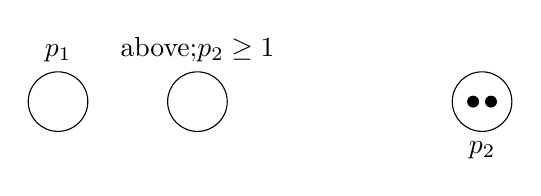
\begin{tikzpicture}
  \node[place,label=above:$p_1$] (p1) {};
  \node[place,label=above;$p_2\ge1$,right=of p1] (p2) {};
  \node[place,label=below:$p_2$, right=5cm,tokens=2 ] (p2) {};
\end{tikzpicture}

\newpage
\section{流程图}

% Define block styles
\tikzstyle{decision} = [diamond, draw, fill=blue!20, 
    text width=4.5em, text badly centered, node distance=3cm, inner sep=0pt]
\tikzstyle{block} = [rectangle, draw, fill=blue!20, 
    text width=5em, text centered, rounded corners, minimum height=4em]
\tikzstyle{line} = [draw, -latex']
\tikzstyle{cloud} = [draw, ellipse,fill=red!20, node distance=3cm,
    minimum height=2em]
    
\begin{tikzpicture}[node distance = 2cm, auto]
    % Place nodes
    \node [block] (init) {initialize model};
    \node [cloud, left of=init] (expert) {expert};
    \node [cloud, right of=init] (system) {system};
    \node [block, below of=init] (identify) {identify candidate models};
    \node [block, below of=identify] (evaluate) {evaluate candidate models};
    \node [block, left of=evaluate, node distance=3cm] (update) {update model};
    \node [decision, below of=evaluate] (decide) {is best candidate better?};
    \node [block, below of=decide, node distance=3cm] (stop) {stop};
    % Draw edges
    \path [line] (init) -- (identify);
    \path [line] (identify) -- (evaluate);
    \path [line] (evaluate) -- (decide);
    \path [line] (decide) -| node [near start] {yes} (update);
    \path [line] (update) |- (identify);
    \path [line] (decide) -- node {no}(stop);
    \path [line,dashed] (expert) -- (init);
    \path [line,dashed] (system) -- (init);
    \path [line,dashed] (system) |- (evaluate);
\end{tikzpicture}

\newpage
\section{smartDiagram}

\begin{centger}
\smartdiagram[circular diagram]{circular, 存储管理子系统, {Rexit, aaa}}
\smartdiagram[flow diagram]{flow, {b, c}, d}
\smartdiagram[descriptive diagram]{descriptive,{b,c},d}
\smartdiagram[priority descriptive diagram]{priority descriptive,{b,c},d}
\smartdiagram[bubble diagram]{bubble diagram,{b,c},d,e,f}
\smartdiagram[constellation diagram]{constellation diagram,{b,c},d,e,f}
\smartdiagram[connected constellation diagram]{connected constellation, {b, c},d,e,f}
\smartdiagram[sequence diagram]{sequence, {b, c},d,e,f}
\end{center}

\newpage
\section{脑图}
\begin{center}
\tikz[mindmap,concept color=red, text=black]
\node [concept] {装修}
[clockwise from =0]
child[concept color=blue,text=white]{
  node[concept]{卧室\\主卧}
}
child{
  node[concept]{卧室\\次卧1}
  child{node[concept]{床}}
  child{node[concept]{窗帘}}
}
child[concept color=blue, text=white]{
  node[concept]{卧室\\次卧2}
}
child[concept color=red, text=white]{
  node[concept]{厨房}
}
child[concept color=red, text=white]{
  node[concept]{餐厅}
}
\end{center}

\newpage
\section{折纸}
% 6面筛
\sffamily\scriptsize
\tikz \pic [transform shape,folding line length=15mm, numbered faces
%% face 1={ \node {1};},
%% face 2={ \node {2};},
%% face 3={ \node {3};},
%% face 4={ \node {4};},
%% face 5={ \node {5};},
%% face 6={ \node {6};},
] {cube folding}; % 不同的folding类型有不同的面数和面形状

\tikz \pic [transform shape, folding line length=15mm, numbered faces] {octahedron folding};
\tikz \pic [transform shape, folding line length=15mm, numbered faces] {dodecahedron folding};
\tikz \pic [transform shape, folding line length=15mm, numbered faces] {dodecahedron' folding}; %% 另一个12面折法
\tikz \pic [transform shape, folding line length=15mm, numbered faces] {icosahedron folding}; 

\newpage
% 一个12面日历
\sffamily\scriptsize
\tikz \pic [
transform shape,
every calendar/.style={
at={(-8ex,4ex)},
week list,
month label above centered,
month text=\bfseries\textcolor{red}{\%mt} \%y0,
if={(Sunday) [black!50]}
},
folding line length=2.5cm,
face 1={ \calendar [dates=2017-01-01 to 2017-01-last];},
face 2={ \calendar [dates=2017-02-01 to 2017-02-last];},
face 3={ \calendar [dates=2017-03-01 to 2017-03-last];},
face 4={ \calendar [dates=2017-04-01 to 2017-04-last];},
face 5={ \calendar [dates=2017-05-01 to 2017-05-last];},
face 6={ \calendar [dates=2017-06-01 to 2017-06-last];},
face 7={ \calendar [dates=2017-07-01 to 2017-07-last];},
face 8={ \calendar [dates=2017-08-01 to 2017-08-last];},
face 9={ \calendar [dates=2017-09-01 to 2017-09-last];},
face 10={\calendar [dates=2017-10-01 to 2017-10-last];},
face 11={\calendar [dates=2017-11-01 to 2017-11-last];},
face 12={\calendar [dates=2017-12-01 to 2017-12-last];}
] {dodecahedron folding};


\newpage
\section{分形图}
\pgfdeclarelindenmayersystem{Koch curve}{
  \rule{F -> F-F++F-F}}
\pgfdeclarelindenmayersystem{Sierpinski triangle}{
  \rule{F -> G-F-G}
  \rule{G -> F+G+F}}
\pgfdeclarelindenmayersystem{Fractal plant}{
  \rule{X -> F-[[X]+X]+F[+FX]-X}
  \rule{F -> FF}}
\pgfdeclarelindenmayersystem{Hilbert curve}{
  \rule{L -> +RF-LFL-FR+}
  \rule{R -> -LF+RFR+FL-}}

\begin{tabular}{cc}
\begin{tikzpicture}
\shadedraw[shading=color wheel] 
[l-system={Koch curve, step=2pt, angle=60, axiom=F++F++F, order=4}]
lindenmayer system -- cycle;
\end{tikzpicture}
&
\begin{tikzpicture}
\shadedraw [top color=white, bottom color=blue!80, draw=blue!80!black]

[l-system={Sierpinski triangle, step=2pt, angle=60, axiom=F, order=8}]
lindenmayer system -- cycle;
\end{tikzpicture}
\\
\begin{tikzpicture}
      \shadedraw [bottom color=white, top color=red!80, draw=red!80!black]
    [l-system={Hilbert curve, axiom=L, order=5, step=8pt, angle=90}]
    lindenmayer system; 
\end{tikzpicture}
&
\begin{tikzpicture}
    \draw [green!50!black, rotate=90]
    [l-system={Fractal plant, axiom=X, order=6, step=2pt, angle=25}]
    lindenmayer system; 
\end{tikzpicture}
\end{tabular}

\section{自定义缩放}
  \begin{center}
    \scalebox{0.7}{
      \smartdiagram[descriptive diagram]{
        {单机软件, 在一台机器上运行的软件},
        {C/S软件, 分为客户端和服务端},
        {B/S软件, 无客户端软件,使用浏览器作为客户端},
        {集群, 多台主机部署相同的服务端,共同支持用户服务},
        {分布式, 多台主机部署不同的服务,公共支持用户服务},
        {云, 集合了集群和分布式的特性,所有数据和应用都在服务端},
      }
    }
  \end{center}


\end{document}